\chapter{绪论}\label{ch:1}
\SourcePage{15}

偏微分方程的数值逼近是数值分析的一个重要分支.要作这类逼近,往往需要从多方面了解所研究的问题.

首先,需要了解问题的物理背景,才能理解预期解的行为.这往往有助于选取合适的数值方法.

其次,应当考虑以变分形式(弱形式)表述问题的现代方法,因为这样便可以在 Hilbert 或 Banach 函数空间中寻找广义解.变分方法可以给出解的先验估计,由此可以判断,采用某种数值方法所得到的解有望在哪些范数下证明其稳定性.此外,关于数学问题的解的光滑性结果,可为选择数值方法提供依据,进而决定所能达到的精度.这个精度由误差分析给出.

显然,在选择任何一种数值方法时,都应特别关注与之相关的算法问题.

本书旨在阐明偏微分方程数值逼近的一般思想.现有的方法显然无法一一涉及.我们主要讨论用来离散空间导数的变分数值方法,以及用来对非定常问题作时间推进的有限差分法和分步法.

只要条件允许,我们就揭示乍看各异的数值策略背后的统一思想,给出分析这些方法的一般理论,并结合手头问题的代数结构,介绍可用于实际计算其数值解的多种算法.因此,我们尽量避免采用只在极特殊情形下奏效,或缺乏坚实理论依据的技术细节、技巧和算法.有些问题和方法需要逐一讨论,但在许多情况下,我们会将它们纳入同一个逻辑单元,如一章或一节.

\section{数值逼近的基本思路}\label{sec:1.1}
\SourcePage{16}

我们将考虑大量数学问题及其数值求解方法.对任意给定的边值问题,\figref{fig:1.1.1}示意了作数值逼近时需要依次作出的选择.

层次 [1] 是所研究的边值问题,采用已计及给定边界条件的弱形式.

层次 [2] 给出可选的离散方式,也就是用来将给定问题化为有限维问题的数值方法.所选策略自然会决定数值问题的结构.

本书主要考虑两类离散方法.第一类是 Galerkin 方法及其重要变体 Petrov--Galerkin 方法,它们以微分问题的积分形式为基础.第二类是配置法,即要求微分方程在计算域内选定的一些点上成立.随后,我们将配置法改写成广义 Galerkin 形式,具体做法是把 Galerkin 方法同采用 Gauss 求积公式计算积分的做法结合起来.

我们也会用较少篇幅讨论空间离散的有限差分格式,主要针对非线性对流--扩散方程和波传播问题.对于波传播问题,还将介绍基于有限体积法的途径,这种方法在计算流体动力学中十分常用.

最后,我们将简述区域分解法的基本原理.在科学计算中,这种方法对于并行求解大规模问题最有前景.

文献中也常见其他途径,本书只会在相关处顺带提及.

层次 [3] 指定逼近所用子空间的性质.典型地,有限元法采用低次分片多项式函数,而谱方法采用高次整体代数多项式.我们会讨论并分析这两种重要方法的一些变体,包括混合有限元法和 Legendre、Chebyshev 谱配置法.这个层次的选择决定数值解的函数结构及所能达到的精度,也影响所得代数方程组的拓扑结构.

层次 [4] 要选取合适的算法求解代数问题,尽可能利用相关矩阵的拓扑结构和性质.我们将介绍当时可用于求解大规模对称和非对称方程组的各种重要方法,其中也包括对预处理和多重网格技术的简要介绍.
\SourcePage{17}

\begin{figure}[htbp]
  \centering
  \includegraphics[page=17,pagebox=cropbox,trim=61.83bp 394.33bp 64.17bp 85.00bp,clip,width=.722\paperwidth]{../input/source/Numerical Approximation of Partial Differential Equations.pdf}
  \caption{数值逼近的基本思路}\label{fig:1.1.1}
\end{figure}

对于初边值问题,还要在层次 [1] 和 [2] 之间作时间离散.常用的做法是以有限差商逼近时间导数.也可以采用其他方法,特别是当微分算子的结构比较复杂时.例如,可采用分步策略,将算子拆分为若干部分,各自独立地作时间推进.本书将详细考察有限差分法和分步法,并简要提及其他策略,如间断有限元法、特征 Galerkin 格式和 Taylor--Galerkin 格式.

最后要指出的是,本书\BookRef{part:1}{第一部分}将沿\figref{fig:1.1.1}所示流程的反方向展开,也就是自下而上.我们从层次 [4] 回溯到层次 [2]：先介绍线性代数方程组的求解算法(第~\BookRef{ch:2}{2}~章),再讨论有限元逼近(第~\BookRef{ch:3}{3}~章)和多项式逼近(第~\BookRef{ch:4}{4}~章)的基本概念.第~\BookRef{ch:5}{5}~章将介绍层次 [2] 的离散方法以及时间差分方法.届时我们还会给出三个边值问题的例子,供读者作具体参考.

本书给出的所有数值结果,均在一台主频为 50\,MHz、内存为 128\,MB 的 IBM RISC 560 上以双精度计算得到.该机的峰值性能为 100\,MFlops(LINPACK 测得 31\,MFlops,TPP 测得 84\,MFlops).所用编译器为 IBM AIX XL FORTRAN/6000 2.3 版.

\section{预备记号与函数空间}\label{sec:1.2}
\SourcePage{18}

本节介绍一些后文经常用到的定义和记号.完整的阐述可参见\BookCite{yosida1974}{Yosida(1974)}或\BookCite{brezis1983}{Brezis(1983)}.\BookCite{brezzi-gilardi1987}{Brezzi 和 Gilardi(1987)}也给出了全面、易读的介绍,其中略去了证明.

\medskip
\noindent\textit{(i)Hilbert 空间和 Banach 空间}

设 \(V\) 是一个实线性空间.
\begin{definition*}[内积]
\(V\) 上的{\heiti 内积}是一个双线性映射 \((\cdot,\cdot)\colon V\times V\to\mathbb R\).对任意 \(w,v\in V\),有 \((w,v)=(v,w)\)(对称性).对任意 \(v\in V\),有 \((v,v)\ge 0\)(非负性),且 \((v,v)=0\) 当且仅当 \(v=0\).
\end{definition*}

\begin{definition*}[半范数与范数]
{\heiti 半范数}是一个映射 \(\|\cdot\|\colon V\to\mathbb R\),满足
\[
  \|v\|\ge 0\quad(v\in V),\qquad
  \|cv\|=|c|\|v\|\quad(c\in\mathbb R,\ v\in V),
\]
以及三角不等式 \(\|w+v\|\le\|w\|+\|v\|\)(\(w,v\in V\)).

\(V\) 上的{\heiti 范数}是还满足下述条件的半范数：\(\|v\|=0\) 当且仅当 \(v=0\).如果存在两个正常数 \(M_1\) 和 \(M_2\),使得
\[
  M_1\|v\|\le \lVert\!\lvert v\rvert\!\rVert\le M_2\|v\|
  \qquad (v\in V),
\]
就称 \(V\) 上的两个范数 \(\|\cdot\|\) 和 \(\lVert\!\lvert\cdot\rvert\!\rVert\) 等价.
\end{definition*}

容易验证,任何内积都可通过 \(\|v\|:=(v,v)^{1/2}\) 诱导一个范数.此外,任何范数都可诱导一个距离 \(d(w,v):=\|w-v\|\).

\begin{definition*}[Hilbert 空间与 Banach 空间]
赋予内积的线性空间 \(V\) 称为预 Hilbert 空间,赋予范数的线性空间称为赋范空间.称赋范空间 \(V\) 中的序列 \(v_n\) 为 Cauchy 序列,是指它关于距离 \(d(w,v)=\|w-v\|\) 满足 Cauchy 条件.如果预 Hilbert 空间(分别为赋范空间)\(V\) 中的每个 Cauchy 序列都收敛,则称 \(V\) 为 {\heiti Hilbert 空间}(分别为 {\heiti Banach 空间}).
\end{definition*}

在 Hilbert 空间中,\emph{Schwarz 不等式}成立：
\begin{equation}\label{eq:1.2.1}
  |(w,v)|\le\|w\|\|v\| \qquad (w,v\in V).
\end{equation}

\medskip
\noindent\textit{(ii)对偶空间}

设 \((V,\|\cdot\|_V)\) 和 \((W,\|\cdot\|_W)\) 是赋范空间.用 \(\mathcal L(V;W)\) 表示从 \(V\) 到 \(W\) 的连续线性映射全体.对 \(L\in\mathcal L(V;W)\),定义范数
\begin{equation}\label{eq:1.2.2}
  \|L\|_{\mathcal L(V;W)}:=
  \sup_{\substack{v\in V\\v\ne 0}}\frac{\|Lv\|_W}{\|v\|_V}.
\end{equation}
这样,\(\mathcal L(V;W)\) 是一个赋范空间.如果 \(W\) 是 Banach 空间,\(\mathcal L(V;W)\) 也是 Banach 空间.若 \(W=\mathbb R\),则称 \(\mathcal L(V;\mathbb R)\) 为 \(V\) 的\emph{对偶空间},记作 \(V'\).

\SourcePage{19}
从 \(V'\times V\) 到 \(\mathbb R\) 的双线性形式 \(\langle\cdot,\cdot\rangle\) 由 \(\langle L,v\rangle:=L(v)\) 定义,称为 \(V'\) 与 \(V\) 之间的\emph{对偶配对}.由 Riesz 表示定理(例如,见\BookCite{yosida1974}{Yosida(1974)}第 90 页)可知,若 \(V\) 是 Hilbert 空间,则其对偶空间 \(V'\) 也是 Hilbert 空间,且可与 \(V\) 作典范等同.

\medskip
\noindent\textit{(iii)弱收敛与弱\ensuremath{^*}收敛}

在赋范空间 \(V\) 中,可以引入另一种收敛,即\emph{弱收敛}.
\begin{definition*}[弱收敛]
如果对每个 \(L\in V'\),都有 \(L(v_n)\) 收敛到 \(L(v)\),就称序列 \(v_n\) 弱收敛到 \(v\in V\).
\end{definition*}
可以证明,弱极限 \(v\) 若存在,必唯一.显然,若 \(v_n\) 在 \(V\) 的范数意义下收敛到 \(v\),它也弱收敛到 \(v\).反过来,弱收敛一般不能推出范数收敛,而在有限维空间中两者等价.

在对偶空间 \(V'\) 中,还可以引入第三种收敛,即\emph{弱\ensuremath{^*}收敛}.
\begin{definition*}[弱\ensuremath{^*}收敛]
如果对每个 \(v\in V\),都有 \(L_n(v)\) 收敛到 \(L(v)\),就称泛函序列 \(L_n\in V'\) 弱\(^*\)收敛到 \(L\in V'\).
\end{definition*}
弱\(^*\)极限 \(L\) 若存在,也必唯一.此外,可以证明,\(V'\) 中的弱收敛蕴含弱\(^*\)收敛.

\medskip
\noindent\textit{(iv)\ensuremath{L^p} 空间}

现在引入作为现代偏微分方程理论基础的几个函数空间.设 \(\Omega\) 是 \(\mathbb R^d\)(\(d\ge 1\))中的开集,在 \(\Omega\) 上考虑 Lebesgue 测度.下面是一族很重要的 Banach 空间.设 \(1\le p\le\infty\),考虑满足下列条件的可测函数 \(v\)：
\begin{equation}\label{eq:1.2.3}
  \int_\Omega |v(\boldsymbol{x})|^p\,\mathrm dx<\infty,\qquad 1\le p<\infty,
\end{equation}
或在 \(p=\infty\) 时,
\begin{equation}\label{eq:1.2.4}
  \sup\bigl\{|v(\boldsymbol{x})|\mid\boldsymbol{x}\in\Omega\bigr\}<\infty.
\end{equation}
这些空间通常记作 \(L^p(\Omega)\),相应的范数为
\begin{equation}\label{eq:1.2.5}
  \|v\|_{L^p(\Omega)}:=\left(\int_\Omega |v(\boldsymbol{x})|^p\,\mathrm dx\right)^{1/p},
  \qquad 1\le p<\infty,
\end{equation}
或在 \(p=\infty\) 时,
\begin{equation}\label{eq:1.2.6}
  \|v\|_{L^\infty(\Omega)}:=\sup\bigl\{|v(\boldsymbol{x})|\mid\boldsymbol{x}\in\Omega\bigr\}.
\end{equation}

更准确地说,\(L^p(\Omega)\) 是满足\eqref{eq:1.2.3}或\eqref{eq:1.2.4}的可测函数按如下等价关系所分成的等价类构成的空间：若 \(w\) 和 \(v\) 仅在一个零测集上有差异,则 \(w\equiv v\).换言之,在 \(L^p(\Omega)\) 中,仅在零测集上有差异的两个函数视为同一个元素.因此,\eqref{eq:1.2.4}中对 \(L^\infty(\Omega)\) 的定义及\eqref{eq:1.2.6}中的范数应作如下修改.\SourcePage{20}若
\[
  \inf\bigl\{M\ge 0\mid |v(\boldsymbol{x})|\le M\ \text{在 \(\Omega\) 上几乎处处成立}\bigr\}<\infty,
\]
则 \(v\in L^\infty(\Omega)\),并且
\begin{equation}\label{eq:1.2.7}
  \|v\|_{L^\infty(\Omega)}
  :=\inf\bigl\{M\ge 0\mid |v(\boldsymbol{x})|\le M\ \text{在 \(\Omega\) 上几乎处处成立}\bigr\}.
\end{equation}
这里,“在 \(\Omega\) 上几乎处处成立”意为“除 \(\Omega\) 中的一个零测集外均成立”.

\(L^2(\Omega)\) 是 Hilbert 空间,其内积为
\[
  (w,v)_{L^2(\Omega)}:=\int_\Omega w(\boldsymbol{x})v(\boldsymbol{x})\,\mathrm d\boldsymbol{x}.
\]
出于后文将会说明的原因,\(L^2(\Omega)\) 中的范数记作 \(\|\cdot\|_{0,\Omega}\),在不会混淆区域 \(\Omega\) 时简记作 \(\|\cdot\|_0\).类似地,内积 \((\cdot,\cdot)_{L^2(\Omega)}\) 常记作 \((\cdot,\cdot)_{0,\Omega}\),或简记作 \((\cdot,\cdot)\).

若 \(1\le p<\infty\),则 \(L^p(\Omega)\) 的对偶空间是 \(L^{p'}(\Omega)\),其中 \(1/p+1/p'=1\)(\(p=1\) 时 \(p'=\infty\)).此外,Hölder 不等式成立：
\begin{equation}\label{eq:1.2.8}
  \left|\int_\Omega w(\boldsymbol{x})v(\boldsymbol{x})\,\mathrm d\boldsymbol{x}\right|
  \le \|w\|_{L^p(\Omega)}\|v\|_{L^{p'}(\Omega)}.
\end{equation}
注意,\(p=2\) 时,Hölder 不等式就是 Hilbert 空间 \(L^2(\Omega)\) 中的 Schwarz 不等式\eqref{eq:1.2.1}.

由\eqref{eq:1.2.8}还容易得出,若 \(p\le q\) 且 \(\Omega\) 的测度有限,则 \(L^q(\Omega)\subset L^p(\Omega)\).

\medskip
\noindent\textit{(v)分布}

回顾一下,\(C^\infty_0(\Omega)\)(或 \(\mathcal D(\Omega)\))表示具有紧支集的无穷可微函数组成的空间.也就是说,对其中的每个函数,都存在一个与 \(\partial\Omega\) 相距为正的有界开集 \(\Omega'\subset\Omega\),使函数在 \(\Omega'\) 外为零.

给出 \(\mathcal D(\Omega)\) 中序列的收敛概念很有用.如果存在闭有界集 \(K\subset\Omega\),使每个 \(v_n\) 在 \(K\) 外为零,并且对每个非负多重指标 \(\boldsymbol{\alpha}\),导数 \(D^{\boldsymbol{\alpha}}v_n\) 在 \(\Omega\) 上一致收敛到 \(D^{\boldsymbol{\alpha}}v\),就称序列 \(v_n\in\mathcal D(\Omega)\) 收敛到 \(v\in\mathcal D(\Omega)\).回顾一下,若 \(\boldsymbol{\alpha}=(\alpha_1,\ldots,\alpha_d)\),各 \(\alpha_i\) 都是非负整数,则
\[
  D^{\boldsymbol{\alpha}}v:=
  \frac{\partial^{|\boldsymbol{\alpha}|}v}
       {\partial x_1^{\alpha_1}\cdots\partial x_d^{\alpha_d}},
\]
其中 \(|\boldsymbol{\alpha}|:=\alpha_1+\cdots+\alpha_d\) 是多重指标 \(\boldsymbol{\alpha}\) 的长度.

\begin{definition*}[分布]
在 \(\mathcal D(\Omega)\) 上、关于上述收敛连续的线性泛函全体记作 \(\mathcal D'(\Omega)\),其元素称为{\heiti 分布}.若 \(L\in\mathcal D'(\Omega)\),\(v\in\mathcal D(\Omega)\),通常用对偶配对 \(\langle L,v\rangle\) 表示 \(L(v)\).
\end{definition*}

容易看出,每个函数 \(w\in L^p(\Omega)\) 都对应于如下分布：
\SourcePage{21}
\[
  v\longmapsto \int_\Omega w(\boldsymbol{x})v(\boldsymbol{x})\,\mathrm d\boldsymbol{x},
  \qquad v\in\mathcal D(\Omega).
\]
然而,Dirac 泛函
\[
  v\longmapsto \delta(v):=v(0),\qquad v\in\mathcal D(\mathbb R),
\]
是一个不能用 \(L^p(\mathbb R)\) 中的任何函数表示的分布.

现在可以引入分布的\emph{导数}.
\begin{definition*}[分布导数]
设 \(\boldsymbol{\alpha}\) 是非负多重指标,\(L\) 是一个分布.则 \(D^{\boldsymbol{\alpha}}L\) 是按下式定义的分布：
\begin{equation}\label{eq:1.2.9}
  \langle D^{\boldsymbol{\alpha}}L,v\rangle
  :=(-1)^{|\boldsymbol{\alpha}|}\langle L,D^{\boldsymbol{\alpha}}v\rangle
  \qquad \forall v\in\mathcal D(\Omega).
\end{equation}
\end{definition*}
由此定义可知,分布可以无穷次求导.另一方面,若 \(L\) 由光滑函数给出,通过分部积分容易验证,分布意义下的导数与通常的导数一致.

还要记住,Dirac 分布 \(\delta\) 是 Heaviside 函数的分布导数,其中
\[
  H(x):=\begin{cases}
    1,&x\ge 0,\\
    0,&x<0.
  \end{cases}
\]

最后,若存在 \(g_{\boldsymbol{\alpha}}\in L^p(\Omega)\),使得
\begin{equation}\label{eq:1.2.10}
  \langle D^{\boldsymbol{\alpha}}L,v\rangle
  =\int_\Omega g_{\boldsymbol{\alpha}}(\boldsymbol{x})v(\boldsymbol{x})\,\mathrm d\boldsymbol{x}
  \qquad \forall v\in\mathcal D(\Omega),
\end{equation}
就称分布 \(L\) 的 \(\boldsymbol{\alpha}\) 阶导数是一个属于 \(L^p(\Omega)\) 的函数.

\medskip
\noindent\textit{(vi)Sobolev 空间}

最后介绍另一类函数空间.后文将最常用到这类空间,因为它们是建立偏微分方程变分理论的自然框架.对这些空间的详细阐述可见\BookCite{adams1975}{Adams(1975)}.

\begin{definition*}[Sobolev 空间]
设 \(k\) 为非负整数,\(1\le p\le\infty\).{\heiti Sobolev 空间} \(W^{k,p}(\Omega)\) 由那些属于 \(L^p(\Omega)\)、且直至 \(k\) 阶的全部分布导数都属于 \(L^p(\Omega)\) 的函数 \(v\) 构成.简记为
\begin{equation}\label{eq:1.2.11}
  W^{k,p}(\Omega):=
  \bigl\{v\in L^p(\Omega)\mid
    D^{\boldsymbol{\alpha}}v\in L^p(\Omega)
    \text{ 对每个满足 \(|\boldsymbol{\alpha}|\le k\) 的非负多重指标 \(\boldsymbol{\alpha}\) 成立}
  \bigr\}.
\end{equation}
\end{definition*}

显然,对每个 \(1\le p\le\infty\),都有 \(W^{0,p}(\Omega)=L^p(\Omega)\),而当 \(k_1\le k_2\) 时,有 \(W^{k_2,p}(\Omega)\subset W^{k_1,p}(\Omega)\).当 \(1\le p<\infty\) 时,\(W^{k,p}(\Omega)\) 关于下列范数是 Banach 空间：
\SourcePage{22}
\begin{equation}\label{eq:1.2.12}
  \|v\|_{k,p,\Omega}:=
  \left(\sum_{|\boldsymbol{\alpha}|\le k}\|D^{\boldsymbol{\alpha}}v\|_{L^p(\Omega)}^p\right)^{1/p}.
\end{equation}
此外,它的半范数定义为
\begin{equation}\label{eq:1.2.13}
  |v|_{k,p,\Omega}:=
  \left(\sum_{|\boldsymbol{\alpha}|= k}\|D^{\boldsymbol{\alpha}}v\|_{L^p(\Omega)}^p\right)^{1/p}.
\end{equation}
另一方面,\(W^{k,\infty}(\Omega)\) 关于范数
\begin{equation}\label{eq:1.2.14}
  \|v\|_{k,\infty,\Omega}:=
  \max_{|\boldsymbol{\alpha}|\le k}\|D^{\boldsymbol{\alpha}}v\|_{L^\infty(\Omega)}
\end{equation}
是 Banach 空间,相应的半范数记为
\begin{equation}\label{eq:1.2.15}
  |v|_{k,\infty,\Omega}:=
  \max_{|\boldsymbol{\alpha}|=k}\|D^{\boldsymbol{\alpha}}v\|_{L^\infty(\Omega)}.
\end{equation}
特别地,当 \(p=2\) 时,我们用 \(H^k(\Omega)\) 代替 \(W^{k,2}(\Omega)\),用 \(\|\cdot\|_{k,\Omega}\) 和 \(|\cdot|_{k,\Omega}\) 代替 \(\|\cdot\|_{k,2,\Omega}\) 和 \(|\cdot|_{k,2,\Omega}\).若不会产生混淆,还可简记作 \(\|\cdot\|_k\) 和 \(|\cdot|_k\).

注意,\(H^k(\Omega)\) 关于下列内积是 Hilbert 空间：
\begin{equation}\label{eq:1.2.16}
  (w,v)_{k,\Omega}:=\sum_{|\boldsymbol{\alpha}|\le k}
  (D^{\boldsymbol{\alpha}}w,D^{\boldsymbol{\alpha}}v)_{0,\Omega}.
\end{equation}

最后,用 \(W^{k,p}_0(\Omega)\) 表示 \(C^\infty_0(\Omega)\) 关于范数 \(\|\cdot\|_{k,p,\Omega}\) 的闭包,用 \(W^{-k,p'}(\Omega)\) 表示 \(W^{k,p}_0(\Omega)\) 的对偶空间.与前面一样,当 \(p=2\) 时,分别用 \(H^k_0(\Omega)\) 和 \(H^{-k}(\Omega)\) 代替 \(W^{k,2}_0(\Omega)\) 和 \(W^{-k,2}(\Omega)\).

当 \(1\le p<\infty\) 时,还可以证明 \(W^{0,p}_0(\Omega)=L^p(\Omega)\).若 \(\Omega\) 具有 Lipschitz 连续边界,则 \(W^{k,p}(\Omega)\) 是 \(C^\infty(\overline\Omega)\) 关于范数 \(\|\cdot\|_{k,p,\Omega}\) 的闭包.换言之,\(C^\infty(\overline\Omega)\) 在 \(W^{k,p}(\Omega)\) 中\emph{稠密}.

有时需要考虑 \(s\in\mathbb R\)、\(1\le p\le\infty\) 时的 Sobolev 空间 \(W^{s,p}(\Omega)\).这里不展开讨论,只回顾 \(\Omega=\mathbb R^d\) 且 \(p=2\) 的情形.此时可用 Fourier 变换 \(\widehat v(\boldsymbol{\xi})\) 将 \(W^{s,2}(\mathbb R^d)=H^s(\mathbb R^d)\) 刻画如下：
\begin{equation}\label{eq:1.2.17}
  H^s(\mathbb R^d):=
  \bigl\{v\in\mathcal S'(\mathbb R^d)\mid
  (1+|\boldsymbol{\xi}|^2)^{s/2}\widehat v(\boldsymbol{\xi})\in L^2(\mathbb R^d)\bigr\},
\end{equation}
其中 \(\mathcal S'(\mathbb R^d)\) 是缓增分布空间.当 \(s\ge 0\) 时,这个条件蕴含 \(v\in L^2(\mathbb R^d)\).

讨论向量值函数 \(\boldsymbol{v}\colon\Omega\to\mathbb R^d\) 时,还常用空间
\begin{equation}\label{eq:1.2.18}
  H(\operatorname{div};\Omega):=
  \bigl\{\boldsymbol{v}\in(L^2(\Omega))^d\mid\operatorname{div}\boldsymbol{v}\in L^2(\Omega)\bigr\}.
\end{equation}
这个空间赋有图范数,即
\SourcePage{23}
\begin{equation}\label{eq:1.2.19}
  \|\boldsymbol{v}\|_{H(\operatorname{div};\Omega)}:=
  \left(\|\boldsymbol{v}\|_{0,\Omega}^2+\|\operatorname{div}\boldsymbol{v}\|_{0,\Omega}^2\right)^{1/2}.
\end{equation}
与前面的情形类似,若 \(\Omega\) 具有 Lipschitz 连续边界,则可以证明,\(H(\operatorname{div};\Omega)\) 是 \((C^\infty(\overline\Omega))^d\) 关于范数 \(\|\cdot\|_{H(\operatorname{div};\Omega)}\) 的闭包.

另一类重要的 Sobolev 空间是 \(W^{s,p}(\Sigma)\),其中 \(s\ge 0\),\(1\le p\le\infty\),而 \(\Sigma\) 是边界 \(\partial\Omega\) 的适当子集.这些空间的定义需要引入一些技术工具,尤其当 \(\Sigma\) 是非光滑的超曲面时,例如多边形区域的边界.关于这一点,可参见\BookCite{adams1975}{Adams(1975)}或\BookCite{brezzi-gilardi1987}{Brezzi 和 Gilardi(1987)}.我们会在\BookRef{sec:1.3}{1.3}~节回过头来给出这些空间的一种刻画.当 \(\Sigma=\partial\Omega\) 时,\(W^{s,2}(\partial\Omega)=H^s(\partial\Omega)\) 的对偶空间记作 \(H^{-s}(\partial\Omega)\).

考虑时空函数 \(v(t,\boldsymbol{x})\),其中 \((t,\boldsymbol{x})\in Q_T:=(0,T)\times\Omega\).这时自然要引入如下空间：
\begin{equation}\label{eq:1.2.20}
  \begin{split}
    L^q(0,T;W^{s,p}(\Omega)):=\biggl\{v\colon(0,T)\to W^{s,p}(\Omega)\;\bigg|\;
    & v\text{ 可测,且}\\[-2pt]
    & \int_0^T\|v(t)\|_{s,p,\Omega}^q\,\mathrm dt<\infty\biggr\},
  \end{split}
\end{equation}
其中 \(1\le q<\infty\),赋予范数
\begin{equation}\label{eq:1.2.21}
  \|v\|_{L^q(0,T;W^{s,p}(\Omega))}:=
  \left(\int_0^T\|v(t)\|_{s,p,\Omega}^q\,\mathrm dt\right)^{1/q}.
\end{equation}
类似地,可以定义 \(L^\infty(0,T;W^{s,p}(\Omega))\) 和 \(C^0([0,T];W^{s,p}(\Omega))\).

定义 Sobolev 空间 \(W^{r,q}(0,T;W^{s,p}(\Omega))\)(\(r\ge 0\))需要用到一些技术性结果,参见\BookCite{lions-magenes1968a}{Lions 和 Magenes(1968a)}或\BookCite{brezzi-gilardi1987}{Brezzi 和 Gilardi(1987)}.为说明其含义,设 \(V\) 是 Banach 空间,空间 \(H^1(0,T;V)\) 可定义为
\begin{equation}\label{eq:1.2.22}
  H^1(0,T;V):=
  \left\{v\in L^2(0,T;V)\;\middle|\;\frac{\partial v}{\partial t}\in L^2(0,T;V)\right\}.
\end{equation}
这里,\(\partial v/\partial t\) 要理解为取值于 \(V\) 的分布意义下的导数.由于前面只介绍了实值分布,技术上的关键是给这句话赋予精确含义.不过,在若干有意义的情形下,也可以用另一种方式给出定义.例如,当 \(V=L^2(\Omega)\) 时,\(H^1(0,T;L^2(\Omega))\) 由分布意义下的时间导数也在 \(L^2(Q_T)\) 中的 \(L^2(Q_T)\) 函数组成.

\section{Sobolev 空间的若干结果}\label{sec:1.3}
\SourcePage{24}

本节介绍 Sobolev 空间中函数所具有的若干重要性质,略去证明.主要限于 Hilbert 空间 \(H^s(\Omega)\) 的情形.一般情形及所有证明,可参见\BookCite{lions-magenes1968a}{Lions 和 Magenes(1968a}、\BookCite{lions-magenes1968b}{1968b)}或\BookCite{adams1975}{Adams(1975)}.

先从所谓的迹定理说起.粗略地说,函数 \(v\in H^s(\Omega)\) 在边界 \(\partial\Omega\) 上的迹,是 \(v\) 限制在 \(\partial\Omega\) 上的值.事实上,由于 \(H^s(\Omega)\) 中的函数在零测集上的值并不唯一确定,这种说法本身还没有明确的含义.记 \(C^0(\overline\Omega)\) 为 \(\overline\Omega\) 上连续函数组成的空间,则精确的结果如下.

\begin{theorem}[迹定理]{1.3.1}
设 \(\Omega\) 是 \(\mathbb R^d\) 中的有界开集,边界 \(\partial\Omega\) 为 Lipschitz 连续,且 \(1/2<s<3/2\).
\begin{enumerate}[label=\alph*.,leftmargin=*]
  \item 存在唯一的连续线性映射 \(\gamma_0\colon H^s(\Omega)\to H^{s-1/2}(\partial\Omega)\),使得对每个 \(v\in H^s(\Omega)\cap C^0(\overline\Omega)\),都有 \(\gamma_0v=v|_{\partial\Omega}\).
  \item 存在连续线性映射 \(\mathcal R_0\colon H^{s-1/2}(\partial\Omega)\to H^s(\Omega)\),使得对每个 \(\varphi\in H^{s-1/2}(\partial\Omega)\),都有 \(\gamma_0\mathcal R_0\varphi=\varphi\).
\end{enumerate}
如果边界光滑,以上结果对任意 \(s>1/2\) 成立.将迹限制在 \(\partial\Omega\) 的 Lipschitz 边界片 \(\Sigma\) 上,所得迹算子 \(\gamma_\Sigma\) 也具有类似性质.
\end{theorem}

由此可见,\(H^{s-1/2}(\Sigma)\) 中的任一函数都是某个 \(H^s(\Omega)\) 函数在 \(\Sigma\) 上的迹.这就给出了刻画 \(H^{s-1/2}(\Sigma)\) 的一种有用方式.

特别要指出的是,由上述定理可知,存在常数 \(C^*>0\),使得
\begin{equation}\label{eq:1.3.1}
  \int_{\partial\Omega}(\gamma_0v)^2\,\mathrm d\gamma
  \le C^*\int_\Omega (v^2+|\nabla v|^2)\,\mathrm d\boldsymbol{x}
  \qquad \forall v\in H^1(\Omega),
\end{equation}
其中 \(\mathrm d\gamma\) 表示 \(\partial\Omega\) 上的曲面测度.

对于 \(H(\operatorname{div};\Omega)\) 中的向量函数,可以证明下列迹定理.

\begin{theorem}[向量函数的迹定理]{1.3.2}
设 \(\Omega\) 是 \(\mathbb R^d\) 中的有界开集,其边界 \(\partial\Omega\) 为 Lipschitz 连续.
\begin{enumerate}[label=\alph*.,leftmargin=*]
  \item 存在唯一的连续线性映射 \(\gamma^\star\colon H(\operatorname{div};\Omega)\to H^{-1/2}(\partial\Omega)\),使得对每个 \(\boldsymbol{v}\in H(\operatorname{div};\Omega)\cap(C^0(\overline\Omega))^d\),都有 \(\gamma^\star\boldsymbol{v}=(\boldsymbol{v}\cdot\boldsymbol{n})|_{\partial\Omega}\).
  \item 存在连续线性映射 \(\mathcal R^\star\colon H^{-1/2}(\partial\Omega)\to H(\operatorname{div};\Omega)\),使得对每个 \(\varphi\in H^{-1/2}(\partial\Omega)\),都有 \(\gamma^\star\mathcal R^\star\varphi=\varphi\).
\end{enumerate}
\end{theorem}

这里,\(\boldsymbol{n}\) 表示 \(\partial\Omega\) 上的单位外法向量.还应注意,对于 \(\boldsymbol{v}\in H(\operatorname{div};\Omega)\),如果只取边界的一个真子集 \(\Sigma\) 上的法向迹,\SourcePage{25}该迹一般属于比 \(H^{-1/2}(\Sigma)\) 更大的空间,通常记为 \(H^{-1/2}_{00}(\Sigma)\)(例如,见\BookCite{lions-magenes1968a}{Lions 和 Magenes(1968a)}).

借助这些迹算子,可以刻画 \(H^1_0(\Omega)\) 和 \(H_0(\operatorname{div};\Omega):=\overline{(C^\infty_0(\Omega))^d}\),这里的闭包是相对于范数 \(\|\cdot\|_{H(\operatorname{div};\Omega)}\) 而言的.事实上,若边界 \(\partial\Omega\) 为 Lipschitz 连续,则
\[
  H^1_0(\Omega)=\{v\in H^1(\Omega)\mid\gamma_0v=0\},\qquad
  H_0(\operatorname{div};\Omega)
   =\{\boldsymbol{v}\in H(\operatorname{div};\Omega)\mid\gamma^\star\boldsymbol{v}=0\}.
\]
空间
\[
  H^1_\Sigma(\Omega):=\{v\in H^1(\Omega)\mid\gamma_\Sigma v=0\}
\]
也有类似的刻画.

下面是所谓的 Poincaré 不等式.这一重要结果将在后文得到广泛应用.

\begin{theorem}[Poincaré 不等式]{1.3.3}
设 \(\Omega\) 是 \(\mathbb R^d\) 中的有界连通开集,\(\Sigma\) 是其边界 \(\partial\Omega\) 上的非空 Lipschitz 边界片.则存在常数 \(C_\Omega>0\),使得
\begin{equation}\label{eq:1.3.2}
  \int_\Omega v^2(\boldsymbol{x})\,\mathrm d\boldsymbol{x}
  \le C_\Omega\int_\Omega|\nabla v(\boldsymbol{x})|^2\,\mathrm d\boldsymbol{x}
  \qquad \forall v\in H^1_\Sigma(\Omega).
\end{equation}
\end{theorem}

若 \(\partial\Omega\) 为 Lipschitz 连续,由 \(C^\infty(\overline\Omega)\) 在 \(H^1(\Omega)\) 中的稠密性容易证明,对任意 \(w,v\in H^1(\Omega)\),下列 Green 公式成立：
\begin{equation}\label{eq:1.3.3}
  \int_\Omega (D_jw)v\,\mathrm d\boldsymbol{x}
  =-\int_\Omega wD_jv\,\mathrm d\boldsymbol{x}
   +\int_{\partial\Omega}\gamma_0w\,\gamma_0v\,n_j\,\mathrm d\gamma,
  \qquad j=1,\ldots,d,
\end{equation}
其中 \(D_j\) 表示偏导数 \(\partial/\partial x_j\).

类似地,对于 \(\boldsymbol{w}\in H(\operatorname{div};\Omega)\) 和 \(v\in H^1(\Omega)\),有
\begin{equation}\label{eq:1.3.4}
  \int_\Omega(\operatorname{div}\boldsymbol{w})v\,\mathrm d\boldsymbol{x}
  =-\int_\Omega\boldsymbol{w}\cdot\nabla v\,\mathrm d\boldsymbol{x}
   +\langle\gamma^\star\boldsymbol{w},\gamma_0v\rangle_{H^{-1/2}(\partial\Omega),H^{1/2}(\partial\Omega)}.
\end{equation}

如前所述,Sobolev 空间 \(W^{s,p}(\Omega)\) 中的函数在零测集上的值并不唯一确定.然而,只要对指标 \(s\) 和 \(p\) 施加适当限制,这些函数便具有一定的正则性.下面的定理说明了这一点.

\begin{theorem}[Sobolev 嵌入定理]{1.3.4}
设 \(\Omega\) 是 \(\mathbb R^d\) 中边界为 Lipschitz 连续的开集(可有界,也可无界),并设 \(1\le p<\infty\).下列嵌入连续：
\begin{enumerate}[label=\alph*.,leftmargin=*]
  \item 若 \(0\le sp<d\),则 \(W^{s,p}(\Omega)\subset L^{p^*}(\Omega)\),其中 \(p^*=dp/(d-sp)\).
  \item 若 \(sp=d\),则对任意 \(p\le q<\infty\),有 \(W^{s,p}(\Omega)\subset L^q(\Omega)\).
  \item \SourcePage{26}若 \(sp>d\),则 \(W^{s,p}(\Omega)\subset C^0(\overline\Omega)\).
\end{enumerate}
\end{theorem}

回顾一下,两个 Banach 空间之间的映射 \(\Psi\colon X\to Y\),若它连续,且对 \(X\) 中的任意有界序列 \(\{x_n\}\),都能选出子序列 \(\{x_{n_k}\}\),使 \(\Psi(x_{n_k})\) 在 \(Y\) 中收敛,就称它是紧映射.现在可以陈述另一个重要结果,对上述 Sobolev 嵌入作进一步说明.

\begin{theorem}[Rellich--Kondrachov 紧性定理]{1.3.5}
设 \(\Omega\) 是 \(\mathbb R^d\) 中的有界开集,其边界为 Lipschitz 连续,并设 \(1\le p<\infty\).下列嵌入是紧的：
\begin{enumerate}[label=\alph*.,leftmargin=*]
  \item 若 \(0<sp<d\),则对任意 \(1\le q<p^*:=dp/(d-sp)\),有 \(W^{s,p}(\Omega)\subset L^q(\Omega)\).
  \item 若 \(sp=d\),则对任意 \(1\le q<\infty\),有 \(W^{s,p}(\Omega)\subset L^q(\Omega)\).
  \item 若 \(sp>d\),则 \(W^{s,p}(\Omega)\subset C^0(\overline\Omega)\).
  \item 若 \(p>2d/(d+2)\),则 \(L^p(\Omega)\subset H^{-1}(\Omega)\).
\end{enumerate}
特别地,对于非负整数 \(k\),\(H^k(\Omega)\) 紧嵌入 \(H^{k-1}(\Omega)\).
\end{theorem}

注意,\(d>2\) 时,在 a 项中取 \(s=1\)、\(p=2\),从而 \(p^*=2d/(d-2)\),再由 Schauder 对偶定理(见\BookCite{yosida1974}{Yosida(1974)}第 282 页)即可推出 d 项.对于 \(d=2\) 和 \(d=1\),分别由 b 项和 c 项作同样的推导.

在一维情形,由 Sobolev 定理特别可得 \(H^1(\Omega)\subset C^0(\overline\Omega)\).下列插值不等式给出了更精确的 \(C^0\) 范数估计.

\begin{theorem}[Gagliardo--Nirenberg 插值不等式]{1.3.6}
设 \((a,b)\) 是一个有界区间,则有
\[
  \max_{a\le x\le b}|v(x)|
  \le\left(\frac1{b-a}+2\right)^{1/2}\|v\|_0^{1/2}\|v\|_1^{1/2}
  \qquad \forall v\in H^1(a,b).
\]
\end{theorem}

下面给出更一般的插值结果.

\begin{theorem}[插值定理]{1.3.7}
设 \(\Omega\) 是 \(\mathbb R^d\) 中边界为 Lipschitz 连续的开集.设 \(s_1<s_2\) 为两个实数,令 \(r=(1-\theta)s_1+\theta s_2\),其中 \(0\le\theta\le1\).则存在常数 \(C>0\),使得
\[
  \|v\|_r\le C\|v\|_{s_1}^{1-\theta}\|v\|_{s_2}^{\theta}
  \qquad \forall v\in H^{s_2}(\Omega).
\]
\end{theorem}

最后考察适用于时空函数的若干性质.

\begin{theorem}[]{1.3.8}
设 \(\Omega\) 是 \(\mathbb R^d\) 中边界为 Lipschitz 连续的开集,\(s\ge0\) 和 \(r>1/2\) 为实数.则对任意 \(0\le\theta\le1\),空间
\SourcePage{27}
\begin{equation}\label{eq:1.3.5}
  L^2(0,T;H^s(\Omega))\cap H^r(0,T;L^2(\Omega))
\end{equation}
连续嵌入空间
\[
  H^{\theta r}(0,T;H^{(1-\theta)s}(\Omega))\cap C^0([0,T];H^{\sigma_0}(\Omega)),
  \qquad \sigma_0:=\frac{(2r-1)s}{2r}.
\]
如果 \(\Omega\) 还有界且 \(s>0\),则\eqref{eq:1.3.5}定义的空间紧嵌入
\[
  H^{r_1}(0,T;H^{s_1}(\Omega))\cap C^0([0,T];H^{\sigma_1}(\Omega)),
\]
其中 \(s_1\ge0\),\(0\le r_1<r(1-s_1/s)\),且 \(0\le\sigma_1<\sigma_0\).
\end{theorem}

关于插值空间的更多参考资料,例如可见\BookCite{bergh-lofstrom1976}{Bergh 和 Löfström(1976)}.

\section{比较结果}\label{sec:1.4}

本节给出两个比较结果,它们将用于分析初边值问题的稳定性和收敛性.

\begin{lemma}[Gronwall 引理]{1.4.1}
设 \(f\in L^1(t_0,T)\) 是非负函数,\(g\) 和 \(\varphi\) 是 \([t_0,T]\) 上的连续函数.若 \(\varphi\) 满足
\begin{equation}\label{eq:1.4.1}
  \varphi(t)\le g(t)+\int_{t_0}^t f(\tau)\varphi(\tau)\,\mathrm d\tau
  \qquad \forall t\in[t_0,T],
\end{equation}
则
\begin{equation}\label{eq:1.4.2}
  \varphi(t)\le g(t)+
  \int_{t_0}^t f(s)g(s)\exp\!\left(\int_s^t f(\tau)\,\mathrm d\tau\right)\mathrm ds
  \qquad \forall t\in[t_0,T].
\end{equation}
若 \(g\) 还单调不减,则
\begin{equation}\label{eq:1.4.3}
  \varphi(t)\le g(t)\exp\!\left(\int_{t_0}^t f(\tau)\,\mathrm d\tau\right)
  \qquad \forall t\in[t_0,T].
\end{equation}
\end{lemma}

\begin{proof}
令 \(R(t):=\int_{t_0}^t f(\tau)\varphi(\tau)\,\mathrm d\tau\).由\eqref{eq:1.4.1}可知,几乎处处有
\[
  \frac{\mathrm dR}{\mathrm dt}(t)=f(t)\varphi(t)\le f(t)[g(t)+R(t)].
\]
因此
\SourcePage{28}
\begin{equation}\label{eq:1.4.4}
  \begin{aligned}
    &\frac{\mathrm d}{\mathrm dt}
      \left[R(t)\exp\!\left(-\int_{t_0}^t f(\tau)\,\mathrm d\tau\right)\right]\\
    &\quad=\left[\frac{\mathrm dR}{\mathrm dt}(t)-R(t)f(t)\right]
       \exp\!\left(-\int_{t_0}^t f(\tau)\,\mathrm d\tau\right)\\
    &\quad\le f(t)g(t)\exp\!\left(-\int_{t_0}^t f(\tau)\,\mathrm d\tau\right).
  \end{aligned}
\end{equation}
在 \((t_0,t)\) 上对\eqref{eq:1.4.4}积分,得到
\[
  R(t)\exp\!\left(-\int_{t_0}^t f(\tau)\,\mathrm d\tau\right)
  \le\int_{t_0}^t f(s)g(s)\exp\!\left(-\int_{t_0}^s f(\tau)\,\mathrm d\tau\right)\mathrm ds,
\]
从而得到\eqref{eq:1.4.2}.

若 \(g\) 单调不减,则
\[
  \varphi(t)\le g(t)\left[1+
  \int_{t_0}^t f(s)\exp\!\left(\int_s^t f(\tau)\,\mathrm d\tau\right)\mathrm ds\right],
\]
由此得到\eqref{eq:1.4.3}.\hfill\(\square\)
\end{proof}

我们常在下列特殊情形下使用 Gronwall 引理：
\begin{equation}\label{eq:1.4.5}
  g(t)=\varphi(0)+\int_0^t\psi(s)\,\mathrm ds,\qquad \psi(s)\ge0.
\end{equation}

下面是另一个比较结果,对应于 Gronwall 引理的离散情形.

\begin{lemma}[离散 Gronwall 引理]{1.4.2}
设 \(k_n\) 为非负序列,且序列 \(\phi_n\) 满足
\begin{equation}\label{eq:1.4.6}
  \begin{cases}
    \phi_0\le g_0,\\[2pt]
    \displaystyle\phi_n\le g_0+\sum_{s=0}^{n-1}p_s+\sum_{s=0}^{n-1}k_s\phi_s,\qquad n\ge1.
  \end{cases}
\end{equation}
则 \(\phi_n\) 满足
\begin{equation}\label{eq:1.4.7}
  \begin{cases}
    \phi_1\le g_0(1+k_0)+p_0,\\[2pt]
    \displaystyle
    \phi_n\le g_0\prod_{s=0}^{n-1}(1+k_s)+
      \sum_{s=0}^{n-2}p_s\prod_{\tau=s+1}^{n-1}(1+k_\tau)+p_{n-1},\qquad n\ge2.
  \end{cases}
\end{equation}
此外,若 \(g_0\ge0\) 且 \(p_n\ge0\)(\(n\ge0\)),则
\begin{equation}\label{eq:1.4.8}
  \phi_n\le\left(g_0+\sum_{s=0}^{n-1}p_s\right)\exp\!\left(\sum_{s=0}^{n-1}k_s\right),
  \qquad n\ge1.
\end{equation}
\end{lemma}

\SourcePage{29}
\begin{proof}
首先,注意到对每个 \(s\ge0\),都有 \(1+k_s\le\exp(k_s)\),故由\eqref{eq:1.4.7}容易得到\eqref{eq:1.4.8}.此外,由假设立即得到\eqref{eq:1.4.7}的第一式.

在证明\eqref{eq:1.4.7}的第二式之前,先回顾用归纳法容易验证的两个等式：
\begin{equation}\label{eq:1.4.9}
  1+k_0+\sum_{s=1}^n k_s\prod_{\tau=0}^{s-1}(1+k_\tau)
  =\prod_{s=0}^n(1+k_s),\qquad n\ge1,
\end{equation}
以及
\begin{equation}\label{eq:1.4.10}
  \begin{aligned}
    &\sum_{s=1}^n(1+k_s)p_{s-1}
    +\sum_{s=2}^n k_s\sum_{\tau=0}^{s-2}p_\tau\prod_{r=\tau+1}^{s-1}(1+k_r)\\
    &\qquad=\sum_{s=0}^{n-1}p_s\prod_{\tau=s+1}^n(1+k_\tau),\qquad n\ge2.
  \end{aligned}
\end{equation}

\eqref{eq:1.4.7}的第二式也用归纳法证明.事实上,首先有
\[
  \begin{aligned}
    \phi_2
    &\le g_0+p_0+p_1+k_0\phi_0+k_1\phi_1\\
    &\le (1+k_0)g_0+p_0+p_1+k_1[g_0(1+k_0)+p_0]\\
    &=g_0\prod_{s=0}^1(1+k_s)+p_0(1+k_1)+p_1.
  \end{aligned}
\]
也就是说,\(n=2\) 时\eqref{eq:1.4.7}的第二式成立.现假定对每个 \(2\le s\le n\),该式均成立,下面证明它对 \(n+1\) 也成立.我们有
\[
  \begin{aligned}
    \phi_{n+1}
    &\le g_0+\sum_{s=0}^n p_s+\sum_{s=0}^n k_s\phi_s\\
    &\le g_0+p_n+\sum_{s=1}^n p_{s-1}+k_0g_0+k_1[g_0(1+k_0)+p_0]\\
    &\quad+\sum_{s=2}^n k_s\left[
      g_0\prod_{r=0}^{s-1}(1+k_r)+
      \sum_{\tau=0}^{s-2}p_\tau\prod_{r=\tau+1}^{s-1}(1+k_r)+p_{s-1}\right]\\
    &\le g_0\left[(1+k_0)+\sum_{s=1}^n k_s\prod_{r=0}^{s-1}(1+k_r)\right]\\
    &\quad+p_n+\sum_{s=1}^n(1+k_s)p_{s-1}+
      \sum_{s=2}^n k_s\sum_{\tau=0}^{s-2}p_\tau\prod_{r=\tau+1}^{s-1}(1+k_r).
  \end{aligned}
\]
因此,由\eqref{eq:1.4.9}和\eqref{eq:1.4.10}即得所要证明的结论.\hfill\(\square\)
\end{proof}

\SourcePage{30}
更一般的形如\eqref{eq:1.4.7}的不等式,可参见\BookCite{lakshmikantham-trigiante1988}{Lakshmikantham 和 Trigiante(1988)}.
